\documentclass[11pt]{article}
\pdfinfoomitdate=1
\pdftrailerid{}
\pdfsuppressptexinfo=15
\usepackage[T1]{fontenc}
\usepackage{lmodern,amsmath,amssymb,amsthm}
\pdfglyphtounicode{parenleftbig}{0028}
\pdfglyphtounicode{parenrightbig}{0029}
\pdfgentounicode=1
\usepackage[margin=1in]{geometry}
\usepackage{microtype,enumitem,needspace}
\usepackage{tikz}
\usetikzlibrary{arrows.meta}
\usepackage[numbers,sort&compress]{natbib}
\usepackage[colorlinks=true,linkcolor=blue,citecolor=blue,urlcolor=blue]{hyperref}
\newcommand{\doi}[1]{doi: \href{https://doi.org/#1}{\nolinkurl{#1}}}
\newtheorem{theorem}{Theorem}[section]
\newtheorem{lemma}[theorem]{Lemma}
\newtheorem{proposition}[theorem]{Proposition}
\newtheorem{corollary}[theorem]{Corollary}
\theoremstyle{remark}
\newtheorem{remark}[theorem]{Remark}
\newcommand{\ii}{\mathrm i}
\newcommand{\abs}[1]{\left|#1\right|}
\newcommand{\R}{\mathbb R}
\newcommand{\C}{\mathbb C}
\newcommand{\e}{\mathrm e}
\numberwithin{equation}{section}
\setlist{itemsep=3pt,topsep=5pt}
\hypersetup{
 pdftitle={Paired states and Hamiltonian cycles in cubic bipartite planar graphs},
 pdfauthor={OpenAI},
 pdfsubject={A proof of Barnette's conjecture by induced tree partitions}
}
\title{Paired states and Hamiltonian cycles\\
in cubic bipartite planar graphs}
\author{OpenAI}
\date{September 24, 2026}

\begin{document}
\maketitle
\begin{abstract}
We prove Barnette's conjecture: every finite simple cubic bipartite planar
\(3\)-vertex-connected graph has a Hamiltonian cycle.
\end{abstract}

\section{Introduction}

A graph is \emph{cubic} if every vertex has degree three, and
\emph{bipartite} if its vertices can be divided into two classes with
no edge inside either class. It is \emph{\(3\)-vertex-connected} if it
has at least four vertices and deleting any set of at most two vertices
leaves it connected. A \emph{Hamiltonian cycle} visits every vertex
exactly once. We consider finite simple undirected graphs throughout
the main statement.

Barnette's conjecture, recorded by Gr\"unbaum in the 1969 Waterloo
proceedings \cite{Barnette1969}, asserts that every cubic bipartite polyhedral
graph is Hamiltonian, where polyhedral means planar and
\(3\)-vertex-connected. It belongs to the line of questions initiated
by Tait's conjecture for cubic polyhedral graphs, disproved by
Tutte \cite{Tutte1946}; see \citet{APSW2016,GSW2023} for the history
and equivalent formulations.

Several partial results explain the role of face structure.
Goodey proved the case in which all faces are quadrilaterals or
hexagons \cite{Goodey1975}. Feder and Subi allowed arbitrarily
large faces in one class of a proper three-coloring of the faces,
requiring only quadrilaterals and hexagons in the other two classes
\cite{FederSubi2006}. Their argument uses proper quasi spanning trees of faces
after contracting a distinguished face class. Kardo\v{s} proved
the related Barnette--Goodey conjecture for cubic polyhedral graphs
with faces of size at most six, without assuming bipartiteness
\cite{Kardos2020}. More recently, Schnieders proved the
faces-at-most-eight case of Barnette's conjecture
\cite[Corollary~1.13]{Schnieders2025}. We remove the face-size
restriction within the full \(3\)-connected bipartite class.

\begin{theorem}\label{thm:main}
Every finite simple undirected graph that is cubic, bipartite,
planar, and \(3\)-vertex-connected has a Hamiltonian cycle.
\end{theorem}

The difficulty is to obtain one spanning cycle. A spanning subgraph
of degree two can have several cycle components, and local choices
alone need not join them. We instead construct an acyclic edge set
in a dual triangulation whose complement becomes one connected
spanning cycle. The construction also retains a prescribed local
pattern needed when the triangulation is cut into smaller pieces.

\subsection{The dual problem and the proof strategy}

For a graph satisfying Theorem~\ref{thm:main}, the faces of its sphere
dual are triangles.
A bipartition of the original graph colors these triangles black
and white, with opposite colors across every edge. The dual viewpoint goes back to Stein's region-partition formulation
\cite[Theorem~2.2]{Stein1971}. In the form proved by Alt, Payne,
Schmidt, and Wood \cite[Lemma~5]{APSW2016}, Hamiltonicity corresponds
to a partition of the triangulation's vertices into two sets, each
inducing a tree. Here an induced tree includes \emph{every}
edge between its vertices, so connectedness alone is insufficient.
Theorem~\ref{thm:partition} proves this partition with any chosen
facial edge's endpoints in one class and its third vertex in the
other. The corresponding Hamiltonian cycle avoids any specified
single edge, as shown in Corollary~\ref{cor:edge-avoidance}. This
single-edge avoidance property is a known equivalent global
strengthening of Barnette's conjecture, through the work of Kelmans
as explained by Hertel \cite[Corollary~3]{Hertel2005} and by
Gorsky, Steiner, and Wiederrecht \cite[Theorem~4.3]{GSW2023}.
Corollary~\ref{cor:pfaffian-paths} records a further consequence
through their published equivalence \cite[Theorem~4.16]{GSW2023}:
every three-edge path in a finite simple cubic \(3\)-vertex-connected Pfaffian
bipartite graph is contained in a Hamiltonian cycle.

To explain the construction, choose one black triangle as the outer
face and call its three vertices the roots. The remaining black
triangles and the nonroot vertices have equal cardinality. A
\emph{state} assigns each remaining black triangle one of its vertices,
using every nonroot exactly once. These face--vertex incidence
matchings are Tutte states, arising in Tutte's theory of trinity
\cite{Tutte1975}. Hine and K\'alm\'an give a modern treatment and
relate the state moves to Kauffman's clock theorem \cite{HK2018}.
A \emph{pair} consists of two states making distinct
choices at every triangle. We prove all state properties needed here.

For a second state \(s\), let \(Q_s\) contain the edge opposite its
chosen vertex in each remaining black triangle. We seek a pair for which
\(Q_s\) is a forest. When no triangle has vertices strictly on both sides,
a planar density inequality and an integral flow first provide a pair.
A disk count supplies the signed cycle identity used in the next step.

We analyze one finite exponential sum over pairs in two different ways.
First fix \(s\). If \(Q_s\) has a cycle, reversing that cycle changes
only the first state \(r\). The disk identity shows that the two terms
have opposite phases, while their real weights agree because those
weights depend only on \(s\). Thus all pairs with cyclic \(Q_s\) cancel.
To prove that the whole sum is nonzero, instead fix the undirected edge
set \(D\) joining the two chosen vertices in each triangle. Its components
are cycles, and its pairs are exactly their independent orientations.
Here reversal exchanges the two state choices along a cycle. Join each
remaining black-face center to its three vertices by spokes. Positive circulations
on these spokes give real weights for which the counterclockwise
orientation of each cycle has the larger sum of weights.
Each cycle then contributes a simple zero at parameter zero. The disk
identity makes the leading phases agree for groups with the fewest
cycles, and their leading magnitudes are positive. These contributions
cannot cancel. Some pair with \(Q_s\) a forest must remain.

A forest state has one root in each of three components. Complementary
plane-tree duality turns it into a tree on the white faces, which selects
one edge at every black and white face. The disk identity proves these
selected edges acyclic. Their complementary dual is connected and
has degree two everywhere; its two sides identify the required induced
trees. Finally, a separating triangle is shared by two smaller
triangulations. The prescribed facial pattern makes their partitions
agree on that triangle, so the trees glue along a vertex or an edge.

Two established matching constructions help place these steps in
context. The passage between incidence matchings and plane trees
is related to Temperley's correspondence and its weighted extension
by Kenyon, Propp, and Wilson \cite{KPW2000}. Regrouping two matchings
by their union cycles is familiar from the double-dimer model
\cite[Lemma~1]{Kenyon2014}. We use this regrouping together with the
separate fixed-second-state cancellation and positive-circulation
argument proved here; neither cited correspondence is an input to
those conclusions.

The weighted sum is finite and is used for existence. The argument
places no bound on the order or face lengths of the input graph;
it does not assert a polynomial-time construction of the cycle.

\section{Plane trees and the triangulation statement}\label{sec:setup}

All embeddings are on the sphere. After choosing an outer face
we work in the plane, with the point at infinity in that face.
Face lengths count edge-side incidences: a bridge contributes
twice to the length of its incident face. A \emph{sphere
triangulation} here is connected and simple, has at least four
vertices, and has a \(3\)-cycle as the boundary of every face.
A \emph{separating triangle} is a \(3\)-cycle with vertices strictly
on both sides.
A \emph{spanning forest} is an acyclic spanning subgraph, with
isolated vertices allowed. For a vertex set \(U\), the induced subgraph
\(T[U]\) contains every edge of \(T\) with both endpoints in \(U\).
A one-vertex graph is a tree. The plane graphs used for intermediate
dual constructions may have loops or parallel edges, with their usual
edge-side incidences; the triangulations themselves are simple.

\begin{lemma}\label{lem:duality}
Let \(M\) be a connected graph embedded on the sphere.
The duals of the edges complementary to a spanning tree of \(M\)
form a spanning tree of \(M^*\). More generally, the duals of the
edges complementary to a spanning forest of \(M\) form a
connected spanning subgraph of \(M^*\).
\end{lemma}

\begin{proof}
Contract a primal spanning tree to one vertex. Contraction
preserves faces and deletes the corresponding dual edges; the
dual of the remaining connected plane graph is connected.
The complementary dual edges number
\(\abs{E(M)}-\abs{V(M)}+1=\abs{F(M)}-1\), by Euler's formula,
so they form a tree. For a spanning forest, extend it to a
spanning tree; its complementary dual contains the tree just
described.
\end{proof}

\begin{theorem}\label{thm:partition}
Let \(T\) be a sphere triangulation whose faces are colored black
and white so that each edge has one incident face of each color.
For any facial triangle \(t_0\) and any edge \(e_0\) of \(t_0\),
the vertex set admits a partition into two sets, each inducing
a tree, such that the endpoints of \(e_0\) are in one set and
the third vertex of \(t_0\) is in the other.
\end{theorem}

We first prove Theorem~\ref{thm:partition} without separating
triangles. Put \(t_0\) on the outer face and exchange the face
colors if necessary to make it black. Its three vertices are
called the \emph{roots}. Let \(k\) be the number of black faces.
Counting sides of either color and applying Euler's formula gives
\begin{equation}\label{eq:counts}
 \#\{\text{white faces}\}=k,\qquad
 \abs{E(T)}=3k,\qquad \abs{V(T)}=k+2.
\end{equation}
Write \(A\) for the black faces other than \(t_0\), and \(X\)
for the nonroot vertices. Thus \(\abs{A}=\abs{X}=k-1\).

A \emph{state} is a bijection \(r:A\longrightarrow X\) with
\(r(t)\in V(t)\), where \(V(t)\) is the vertex set of the
triangle \(t\). A \emph{pair} is an ordered pair of states
\((r,s)\) such that \(r(t)\ne s(t)\) for every \(t\in A\).
Equivalently, a pair consists of two edge-disjoint perfect
matchings in the bipartite incidence graph on \(A\) and \(X\).
This is the planar state convention of \citet[Section~1]{HK2018},
with black and white exchanged; no vertex three-coloring or clock
theorem is needed below.

\section{Two disjoint states}\label{sec:pairs}

Our first task is to supply two distinct choices at every black face
while using each nonroot vertex exactly once in each choice. The capacity-one
incidence edges below enforce that the two states are disjoint.

\begin{proposition}\label{prop:pairs}
If \(T\) has no separating triangle, then a pair of states exists.
\end{proposition}

\begin{proof}
A degree-two spanning subgraph of the incidence graph splits
into two perfect matchings by alternating its bipartite cycles.
It is therefore enough to prove
\begin{equation}\label{eq:flow}
 \sum_{t\in A}\min\bigl(2,\abs{V(t)\cap S}\bigr)\ge2\abs S
 \qquad(S\subseteq X).
\end{equation}
Indeed, give capacity two to source-to-\(X\) and
\(A\)-to-sink edges, and capacity one to incidences from \(X\)
to \(A\). For a cut placing \(S\subseteq X\) on the source side,
minimizing over the placement of \(A\) gives capacity
\[
 2(\abs X-\abs S)+
 \sum_{t\in A}\min\bigl(2,\abs{V(t)\cap S}\bigr).
\]
Thus \eqref{eq:flow} and integral max-flow give a flow of
\(2\abs X=2\abs A\), and hence the required degree-two subgraph.
The underlying max-flow/min-cut principle is due to
\citet{FF1956}. For completeness, the integral conclusion follows
by starting with zero
flow and augmenting along residual source--sink paths. Every augmentation
has a positive integral bottleneck, so at most \(2\abs X\) augmentations
are needed; if no path remains, the residual vertices reachable from the
source define a cut whose capacity equals the flow value. The displayed
cut bound therefore forces the full value. Every capacity-two outer edge
is saturated, and each capacity-one incidence carries zero or one,
giving degree two at every vertex of the incidence graph.

Let \(U=V(T)\setminus S\); it contains the three roots.
Denote by \(e(U)\) the number of edges in \(T[U]\), and by
\(b(U)\) the number of actual black faces of \(T\) all of whose
vertices belong to \(U\). Include \(t_0\) in the sum in
\eqref{eq:flow}, with contribution zero. If a black triangle
has \(j\) vertices in \(U\), its shortfall from two is
\(\max(0,j-1)\). This is its number of edges in \(T[U]\), minus
one if \(j=3\). Since each edge has exactly one black incident
face, \eqref{eq:counts} shows that \eqref{eq:flow} is equivalent to
\begin{equation}\label{eq:density}
 e(U)-b(U)\le2\abs U-4.
\end{equation}

Consider a connected component \(K\) of \(T[U]\) with \(p\ge4\)
vertices, \(m\) edges, and \(f\) faces, with the inherited
sphere embedding. Every face has boundary length at least three.
Its triangular faces are exactly the actual triangular faces
of \(T\) whose vertices lie in \(K\). To justify the only
delicate direction, a triangular component face is bounded
by a \(3\)-cycle. As the cycle is not separating, one side is
an actual face of \(T\). The component has a vertex off the
cycle, on the other side, so its triangular facial side must
be the actual face. The converse follows because an actual
face contains no vertices or edges in its interior.

Let \(b,w\) count these black and white triangular faces of
\(K\). Each other face region has length \(d\ge4\). Let
\(b',w'\) count all original faces of \(T\) in that region.
Signed edge-side counting gives
\[
 3(b'-w')=\sum_{j=1}^{d}\sigma_j,\qquad
 \sigma_j\in\{-1,1\}.
\]
Internal sides cancel in black/white pairs. This remains true
for repeated boundary edges and for regions containing other
components of \(T[U]\). Consequently
\begin{equation}\label{eq:face-defect}
 \lvert b'-w'\rvert\le d-4.
\end{equation}
For \(d=4\), parity and divisibility by three force the signed
sum to be zero. For \(d=5\), its absolute value is at most
three. For \(d\ge6\), use \(d/3\le d-4\).

The regions of \(K\) partition the original faces of \(T\).
Their total color balance therefore gives
\[
 w-b=\sum_{\text{nontriangular regions}}(b'-w')
       \le\sum_{\text{nontriangular faces}}(d-4).
\]
It follows that
\[
 2m=4f-b-w+\sum_{\text{nontriangular faces}}(d-4)
       \ge4f-2b.
\]
Using \(p-m+f=2\) yields
\begin{equation}\label{eq:component}
 m-b\le2p-4.
\end{equation}

The component containing the roots satisfies
\eqref{eq:component} also when it has three vertices:
it is \(t_0\), with three edges and one actual black face.
Every other component satisfies the weaker bound
\(m-b_{\rm act}\le2p\), where \(b_{\rm act}\) counts its
actual black faces. For \(p\ge4\) this follows from
\eqref{eq:component}, and for smaller \(p\) from simplicity.
Summing over components proves \eqref{eq:density}.
\end{proof}

\section{The disk identity}\label{sec:disk}

The next identity controls both cancellation and the final forest
construction. It records more than a face-color imbalance: the state
bijection fixes exactly how many black faces can lie inside a directed
cycle.

For adjacent vertices \(v,w\), define
\(\delta(v,w)=1\) if the black face of their edge is on the
left when the edge is traversed from \(v\) to \(w\), and
\(\delta(v,w)=-1\) otherwise. Thus \(\delta\) is antisymmetric,
and the counterclockwise sides of a bounded black face have
weight one.

\Needspace{24\baselineskip}
\begin{lemma}[Disk identity]\label{lem:disk}
Let \(r\) be a state. In each \(t\in A\), choose one edge
directed from \(r(t)\) to another vertex of \(t\).
Every simple directed cycle in the chosen edges avoids the
roots. Its \(\delta\)-sum is \(-3\) if it is counterclockwise,
and \(3\) if it is clockwise.
\end{lemma}

\begin{proof}
Only nonroots have outgoing edges, so the cycle avoids the
roots. Its bounded disk contains no root, because the roots
are on the outer-face boundary. Let \(h\) be the cycle length,
\(I\) the number of strictly interior vertices, \(B,W\) the
numbers of black and white faces in the disk, and \(l\) the
number of boundary edges with their black face in the disk.
Euler's formula for the triangulated disk and signed side
counting give, respectively,
\begin{equation}\label{eq:disk-counts}
 B+W=2I+h-2,\qquad 3(B-W)=2l-h.
\end{equation}

The state supplies the additional identity
\begin{equation}\label{eq:matching-disk}
 B=I+l.
\end{equation}
Every strictly interior vertex is matched to an incident
black face in the disk. A boundary vertex is matched to the
black face of its outgoing cycle edge, which lies inside in
exactly the \(l\) counted cases. Conversely every black face
in the disk is matched to an interior or boundary vertex.
There is no double counting: the state is a bijection and
at most one chosen edge comes from each black face.

Equations \eqref{eq:disk-counts}--\eqref{eq:matching-disk}
imply \(2l-h=-3\). This is the weight sum for a
counterclockwise traversal. A clockwise traversal reverses
the signs and has sum \(3\).
\end{proof}

The matching condition in \eqref{eq:matching-disk} is essential.
The conclusion need not hold for arbitrary oriented cycles
of the triangulation.

\section{A weighted cancellation argument}\label{sec:cancellation}

For a state \(s\), let \(Q_s\) be the spanning subgraph of
\(T\) consisting of the edge opposite \(s(t)\) in every
\(t\in A\). These edges are distinct, since every edge of
\(T\) has a unique black incident face.
Figure~\ref{fig:local-triangle}(a) shows the two local edge choices.

\begin{proposition}\label{prop:forest-state}
Whenever at least one pair exists, some pair \((r,s)\) has
\(Q_s\) a forest.
\end{proposition}

We prove this by cancelling all cyclic \(Q_s\)'s from a
weighted sum and then proving that the sum is nonzero.
The cancellation works for arbitrary weights; we will choose them
afterwards to establish nonvanishing.

For now, assign a real number \(a(t,v)\) to each incidence
\(t\in A\), \(v\in V(t)\), and write
\[
 \omega(s)=\sum_{t\in A}a(t,s(t)).
\]
For a pair, direct the edge in \(t\) from \(r(t)\) to
\(s(t)\). Every vertex of \(X\) has one edge in and one
out, so these edges form a union \(D\) of vertex-disjoint
cycles on \(X\). They are distinct even as undirected
edges, since each edge belongs to just one black face.
Thus the cycles are simple. By Lemma~\ref{lem:disk},
\begin{equation}\label{eq:J}
 J(r,s)=\frac13\sum_{t\in A}\delta(r(t),s(t))
 \quad\hbox{is an integer}.
\end{equation}
For real \(x\), define the finite exponential sum
\begin{equation}\label{eq:Z}
 Z(x)=\sum_{(r,s)\ {\rm pair}}
             \ii^{J(r,s)}\exp\bigl(x\omega(s)\bigr).
\end{equation}

\subsection{Cancellation}

\begin{lemma}\label{lem:cancel}
For fixed \(s\) with cyclic \(Q_s\), the terms of
\eqref{eq:Z} having second state \(s\) sum to zero.
\end{lemma}

\begin{proof}
If \(s\) has no partner there is nothing to prove.
Otherwise choose a simple undirected cycle in \(Q_s\),
using \(s\) alone to make this choice.
For a partner \(r\), write \(u(t)\) for the third vertex
of \(t\), other than \(r(t),s(t)\), and orient the
opposite edge from \(r(t)\) to \(u(t)\). Every vertex
has outdegree at most one. The chosen cycle must be
directed: its edges need distinct tails at all its
vertices. In particular it contains no root.

On the triangles supplying this cycle, replace \(r(t)\)
by \(u(t)\), and leave all other assignments unchanged.
Call the new state \(\widetilde r\). This cyclically
permutes the vertices assigned along the cycle, so
\(\widetilde r\) remains a bijection and a partner of \(s\).
It reverses the chosen cycle; applying it again restores
\(r\). Thus it is an involution without fixed points.

On a changed triangle, the three cyclic directions give
\[
 \delta(u(t),s(t))-\delta(r(t),s(t))
      =2\delta(r(t),u(t)).
\]
Lemma~\ref{lem:disk}, applied to the directed opposite-edge
cycle, now yields
\[
 J(\widetilde r,s)-J(r,s)=\pm2.
\]
Hence \(\ii^{J(\widetilde r,s)}=-\ii^{J(r,s)}\).
The exponential weights coincide because \(s\) is fixed.
The involution cancels all terms.
\end{proof}

\subsection{Positive spoke circulations}

We now choose the incidence weights so that the two orientations of each
cycle of \(D\) have strictly ordered weights: the sum of
\(a(t,\mathrm{head})\) is larger in the counterclockwise orientation.
We establish this comparison below by replacing cycle edges with spokes.
Inside each bounded black triangle place a center and join
it to the three vertices by disjoint incidence spokes.
Let \(H_0\) be the resulting plane graph, allowing isolated
vertices.

\Needspace{14\baselineskip}
\begin{lemma}\label{lem:circulation}
There are real numbers \(a(t,v)\) on the spokes of \(H_0\)
such that every counterclockwise simple spoke cycle has
strictly positive weight, where center-to-vertex traversal
has weight \(a(t,v)\) and reverse traversal its negative.
\end{lemma}

\begin{proof}
Work separately in each connected component. Prescribe
signed boundary circulation one on every bounded face and
the negative of their number on the unbounded face, always
traversing with the face on the left. For each bounded face
take a simple path in the connected plane dual to the
unbounded face. Give each crossed edge an antisymmetric
weight contributing one to the face being left and minus
one to the face being entered. Along the path these
contributions cancel at intermediate faces. Summing over
bounded faces realizes the prescribed circulations.
Summing face boundaries inside any counterclockwise simple
cycle cancels internal sides and gives the positive number
of component faces inside it. A component with no bounded
face has no cycle and needs no nonzero weights.
\end{proof}

Fix these weights for the remainder of the proof.

\subsection{Nonvanishing}

Group the pairs in \eqref{eq:Z} by their undirected edge
set \(D\). This uses the two-orientations-per-cycle regrouping
familiar from double-dimer expansions
\cite[Section~3.2.1, Lemma~1]{Kenyon2014}. Such a set determines the edge chosen in every
triangle of \(A\), because every edge belongs to a unique
black face. The pairs in its group are exactly the
independent orientation choices on its cycles: tails
give \(r(t)\), heads give \(s(t)\), and each choice
still gives two bijections on \(X\).

For a cycle \(C\) of \(D\), let \(L_+(C)\) be the sum
of \(a(t,\mathrm{head})\) along its counterclockwise
orientation, and \(L_-(C)\) the corresponding clockwise
sum. We claim
\begin{equation}\label{eq:positive-difference}
 L_+(C)-L_-(C)>0.
\end{equation}
For the counterclockwise traversal, replace each edge
by its two-spoke route from tail through the center of
its black triangle to head, as in Figure~\ref{fig:local-triangle}(b).
Its spoke weight is exactly
\(a(t,\mathrm{head})-a(t,\mathrm{tail})\), so the
closed spoke curve has weight \(L_+(C)-L_-(C)\).

This spoke curve is simple and counterclockwise. Indeed,
there is at most one edge from each black triangle in
\(D\). Distinct detours have disjoint interiors, and
their centers are distinct; the only shared original
vertices are successive vertices of the original cycle.
Moreover the original edge and its detour enclose a
subdisk of the black triangle excluding its third
corner. Sliding the edge across that subdisk is an
isotopy through simple curves. This remains true if
the third corner occurs elsewhere on \(C\). Performing
the slides successively preserves the counterclockwise
orientation. Lemma~\ref{lem:circulation} therefore proves
\eqref{eq:positive-difference}.

\begin{figure}[tb]
  \centering
  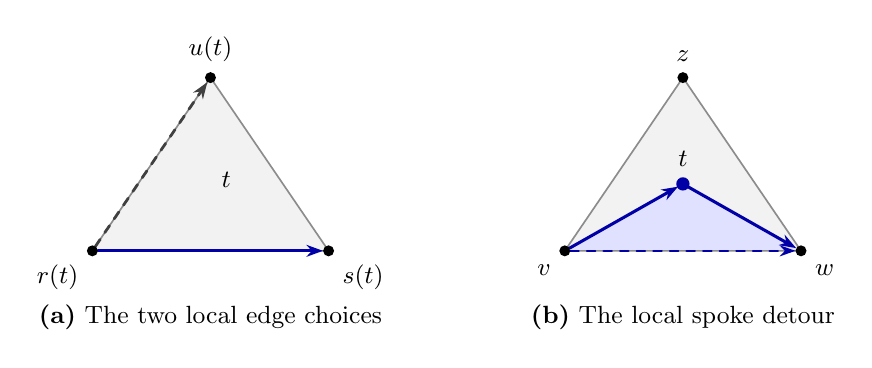
\begin{tikzpicture}[
    font=\small,
    line cap=round,
    line join=round,
    boundary/.style={draw=black!45,line width=.6pt},
    pair edge/.style={draw=blue!65!black,line width=1.1pt,
      -{Stealth[length=2.1mm,width=1.5mm]}},
    opposite edge/.style={draw=black!75,line width=1pt,dashed,
      -{Stealth[length=2.1mm,width=1.5mm]}},
    vertex/.style={circle,fill=black,inner sep=1.4pt}
  ]
    \begin{scope}
      \coordinate (r) at (0,0);
      \coordinate (s) at (3,0);
      \coordinate (u) at (1.5,2.2);
      \fill[black!5] (r)--(s)--(u)--cycle;
      \draw[boundary] (r)--(s)--(u)--cycle;
      \draw[pair edge,shorten >=2pt,shorten <=2pt] (r)--(s);
      \draw[opposite edge,shorten >=2pt,shorten <=2pt] (r)--(u);
      \node[vertex,label=below left:{$r(t)$}] at (r) {};
      \node[vertex,label=below right:{$s(t)$}] at (s) {};
      \node[vertex,label=above:{$u(t)$}] at (u) {};
      \node at (1.7,.9) {$t$};
      \node[align=center] at (1.5,-.85)
        {\textbf{(a)} The two local edge choices};
    \end{scope}
    \begin{scope}[xshift=6cm]
      \coordinate (v) at (0,0);
      \coordinate (w) at (3,0);
      \coordinate (z) at (1.5,2.2);
      \coordinate (c) at (1.5,.85);
      \fill[black!5] (v)--(w)--(z)--cycle;
      \fill[blue!12] (v)--(w)--(c)--cycle;
      \draw[boundary] (v)--(w)--(z)--cycle;
      \draw[draw=blue!65!black,line width=.85pt,dashed,
        -{Stealth[length=2mm,width=1.4mm]},shorten >=2pt,shorten <=2pt]
        (v)--(w);
      \draw[pair edge,shorten >=2pt,shorten <=2pt] (v)--(c);
      \draw[pair edge,shorten >=2pt,shorten <=2pt] (c)--(w);
      \node[vertex,label=below left:{$v$}] at (v) {};
      \node[vertex,label=below right:{$w$}] at (w) {};
      \node[vertex,label=above:{$z$}] at (z) {};
      \node[circle,fill=blue!65!black,inner sep=1.7pt,
        label=above:{$t$}] at (c) {};
      \node[align=center] at (1.5,-.85)
        {\textbf{(b)} The local spoke detour};
    \end{scope}
  \end{tikzpicture}
  \caption{Two local constructions in a bounded black triangle.
    (a) A paired state gives the edge $r(t)\to s(t)$ of $D$
    (solid) and the edge $r(t)\to u(t)$ of $Q_s$ (dashed).
    (b) The directed edge $v\to w$ (dashed) is slid to the
    two-spoke route $v\to t\to w$ (solid), with $t$ denoting
    the face center. The shaded subdisk lies between the two routes
    and excludes the third corner $z$.}
  \label{fig:local-triangle}
\end{figure}


By Lemma~\ref{lem:disk}, a counterclockwise cycle
contributes \(-1\) to \(J\), and a clockwise cycle
contributes \(1\). The whole group contribution is
therefore
\begin{equation}\label{eq:group-product}
 \prod_{C\subset D}
 \left(-\ii\exp(xL_+(C))+\ii\exp(xL_-(C))\right).
\end{equation}
Each factor vanishes to exactly first order at zero.
If \(c(D)\) is the number of cycles of \(D\), the first
nonzero Taylor coefficient of \eqref{eq:group-product}
is in degree \(c(D)\) and equals
\begin{equation}\label{eq:leading-coefficient}
 (-\ii)^{c(D)}
       \prod_{C\subset D}\bigl(L_+(C)-L_-(C)\bigr).
\end{equation}
There is at least one group. In the smallest occurring
degree \(c_{\min}\), all contributing groups have phase
\((-\ii)^{c_{\min}}\) and strictly positive real
magnitudes by \eqref{eq:positive-difference}.
Groups with more cycles have no term of that degree.
Thus this coefficient of \(Z\) is nonzero.
Lemma~\ref{lem:cancel} cancels every second state with
cyclic \(Q_s\), so some pair has \(Q_s\) a forest.
This proves Proposition~\ref{prop:forest-state}.

\section{Recovering the two induced trees}\label{sec:trees}

We now convert the forest state into one selected edge at every face.
The prescription at \(t_0\) enters through the root of a tree on the
white faces. A second use of the disk identity will make the selected
edges acyclic; their complementary dual cycle will establish inducedness.

Assume that \(T\) has no separating triangle.
By Propositions~\ref{prop:pairs} and \ref{prop:forest-state},
choose a pair \((r,s)\) with \(Q_s\) a forest.
Orient its edges from \(r(t)\) to the third vertex.
The outdegrees are one on \(X\) and zero at the roots.
\begin{lemma}\label{lem:root-components}
For a pair \((r,s)\) with \(Q_s\) a forest, every component of
\(Q_s\) contains exactly one of the three roots.
\end{lemma}

\begin{proof}
If a component has \(q\) vertices and \(a\) roots, its total
outdegree is \(q-a\), while its tree edge count is \(q-1\).
Each edge contributes one to the total outdegree, so \(a=1\).
This includes isolated vertices. The partner \(r\) supplies the
orientation and the required outdegrees.
\end{proof}

\subsection{A tree on the white faces}

The construction below uses a relation between matchings and plane
trees, a theme of the Temperley correspondence and its weighted
extension \cite[Theorem~1]{KPW2000}. We give the triangular-state
construction explicitly, including the prescribed outer edge.

Let \(H\) be the sphere graph of incidence spokes from
\emph{all} black centers, including \(t_0\), to their
vertices. This graph is connected, since every edge
of \(T\) can be routed through its black center.
The faces of \(H\) correspond to the white triangles.
To see this, the spokes split each black triangle
into three sectors adjoining its sides. Removing
the original edges of \(T\) joins each white triangle
to the three sectors across its sides, and original
vertices prevent further merging.

Delete the spokes \((t,s(t))\), \(t\in A\).
What remains is the forest \(Q_s\) with its edges
subdivided by their black centers, together with
the three spokes from the center of \(t_0\) to the
three roots. Since those roots lie in distinct
components, the remainder is a spanning tree of \(H\).
By Lemma~\ref{lem:duality}, the duals of the deleted
spokes form a spanning tree on the white triangles.

Root this white-face tree at the white triangle \(y_0\)
across \(e_0\) from \(t_0\). Assign every tree edge to
its endpoint farther from \(y_0\). These endpoints
use each white triangle except \(y_0\) exactly once.
A spoke \((t,v)\) borders the white triangles across
the two sides of \(t\) incident with \(v\).
Thus for the deleted spoke \((t,s(t))\), select the
edge of \(t\) incident with \(s(t)\) bordering its
assigned white triangle. Finally select \(e_0\).

Denote the selected set by \(P\), and put
\(P_0=P\setminus\{e_0\}\).
There is exactly one selected edge at each black
and at each white triangle. Selections from distinct
black faces cannot coincide, so \(\abs P=k\).
Orient each edge of \(P_0\) out from \(s(t)\) in the
black triangle that supplied it.

\subsection{Acyclicity and inducedness}

\begin{lemma}\label{lem:P-forest}
The selected set \(P\) is a forest.
\end{lemma}

\begin{proof}
An undirected simple cycle in \(P_0\) must be
directed, since each vertex has outdegree at most one.
Use \(B,W,h,l\) for its disk data as in
Lemma~\ref{lem:disk}, now with state \(s\).
There is an additional selected-edge count:
\begin{equation}\label{eq:selection-count}
 B-W=2l-h.
\end{equation}
Count the unique selected edge of every interior
face with sign \(+1\) for black and \(-1\) for white.
A selected edge whose relative interior lies inside the disk
contributes one of each sign and cancels. This includes a chord
with both endpoints on the boundary: both of its incident faces
lie in the disk. Every boundary edge
is selected, contributing \(+1\) when its black
face is inside and \(-1\) otherwise. This proves
\eqref{eq:selection-count}.

But signed triangle-side counting gives
\(3(B-W)=2l-h\), so \eqref{eq:selection-count}
would imply \(2l-h=0\). The cycle would therefore have
\(\delta\)-sum zero in either orientation, contrary to
Lemma~\ref{lem:disk}. Thus \(P_0\) is a forest.
Its outdegrees are one at every nonroot and zero at
the roots, so the same component count used for
\(Q_s\) gives one root per component.
The edge \(e_0\) joins two different roots, hence
different components. Adding it preserves acyclicity.
\end{proof}

Take the spanning dual subgraph formed by the edges
dual to \(E(T)\setminus P\). It is connected by
Lemma~\ref{lem:duality}. Every face of \(T\) has two
unselected sides, so this dual subgraph is 2-regular.
It has \(2k>2\) vertices and is one simple cycle.
Draw its edges crossing just their corresponding
primal edges, once transversely, and avoiding all
primal vertices.

The resulting Jordan curve labels each vertex of
\(T\) by the side on which it lies. An edge has
same-label ends exactly when it is in \(P\):
an unselected edge crosses the curve once, while
a selected edge has no crossing. Both labels occur.
By \eqref{eq:counts}, the forest \(P\) has
\((k+2)-k=2\) components. Each has a constant label,
so there is exactly one component for each label.
The classes therefore induce trees. The unique
same-label edge at \(t_0\) is \(e_0\).
This proves Theorem~\ref{thm:partition} in the absence
of separating triangles.

\section{Separating triangles and the Hamiltonian cycle}\label{sec:assembly}

The facial prescription lets us glue partitions across separating
triangles. We then deduce Hamiltonicity and the edge-avoidance consequence.

\begin{proof}[Proof of Theorem~\ref{thm:partition}]
Induct on the number of vertices, using the construction
above when there is no separating triangle.
Otherwise split along a separating \(3\)-cycle into
two sphere triangulations, capping each side by a
triangle on the separating cycle. Both pieces are
simple, have at least four vertices, and are smaller
than \(T\).

The inherited face coloring extends to each cap.
Indeed, on one side let \(B,W\) count its original
black and white faces. Signed side counting makes
\(3(B-W)\) the sum of the three boundary signs,
each \(+1\) or \(-1\). Divisibility by three
forces all three signs to be equal. Color the
cap oppositely.

Apply induction first to the piece containing
the prescribed original face \(t_0\), with its
specified edge \(e_0\). On that piece's cap both
tree labels occur, since a monochromatic triangle
would be a cycle in an induced tree.
Prescribe the same-label edge of the cap in the
other piece and apply induction there. Rename
the two labels to agree on the shared triangle.

For each label the two induced trees intersect
in a connected subtree: one vertex, or one edge
with its endpoints. Their union is a tree.
It is induced in \(T\), since there are no edges
between the interiors of the two sides.
The original prescription is preserved, completing
the induction.
\end{proof}

\begin{proof}[Proof of Theorem~\ref{thm:main}]
Let \(G\) satisfy the four hypotheses and fix a sphere
embedding. It has no edge cut of size one or two.
For otherwise each side of such a cut would have
at least three vertices: cubicity and simplicity
give at least three crossing edges for a singleton
and at least four for two vertices.
Deleting the at most two crossing endpoints on
one side would leave a nonempty remnant disconnected
from the other side, contrary to \(3\)-vertex-connectivity.

The sphere dual \(T=G^*\) is simple. A dual loop
or a pair of parallel dual edges would be a Jordan
curve crossing one or two primal edges once,
giving an edge cut of that size. Its two primal
sides are nonempty, since every crossed edge
has its endpoints on opposite sides.
Cubicity gives each dual face a boundary walk
of length three, which in a simple graph is
a triangle. Euler's formula gives
\(\abs{V(T)}=2+\abs{V(G)}/2\ge4\).
The bipartition of \(G\) colors the faces of \(T\)
black and white with opposite colors at every edge.

Apply Theorem~\ref{thm:partition}. The edges induced
by the two classes form a spanning forest.
Each triangle has exactly one such edge, since
neither tree class can contain all three vertices.
The complementary dual edges in \(G\) are connected
by Lemma~\ref{lem:duality} and give degree two at
every vertex. They form a single spanning cycle,
which is the required Hamiltonian cycle.
\end{proof}

\begin{corollary}\label{cor:edge-avoidance}
For every graph \(G\) satisfying Theorem~\ref{thm:main} and every
edge \(e\in E(G)\), there is a Hamiltonian cycle of \(G\) avoiding \(e\).
\end{corollary}

\begin{proof}
In the dual triangulation choose a facial triangle containing the dual
edge \(e^*\), and prescribe \(e_0=e^*\) in
Theorem~\ref{thm:partition}. That edge belongs to one of the induced
trees. The complementary dual Hamiltonian cycle constructed above
therefore omits \(e\).
\end{proof}

Recall that a graph \(G\) is \emph{Pfaffian} if its edges admit an
orientation for which every even cycle \(C\) such that \(G-V(C)\)
has a perfect matching has an odd number of edges directed along either
cyclic traversal \cite[Section~4]{GSW2023}.

\begin{corollary}[Prescribed paths in Pfaffian graphs]\label{cor:pfaffian-paths}
Let \(G\) be a finite simple undirected graph that is cubic,
\(3\)-vertex-connected, Pfaffian, and bipartite. Every path on four
vertices (three edges) in \(G\) is contained in a Hamiltonian cycle.
In other words, \(G\) is \(P_4\)-Hamiltonian; in particular, it is
Hamiltonian.
\end{corollary}

\begin{proof}
Gorsky, Steiner, and Wiederrecht \cite[Theorem~4.16]{GSW2023} proved
the equivalence of Barnette's conjecture, their condition~(i), with
this \(P_4\)-Hamiltonicity statement, their condition~(v).
Theorem~\ref{thm:main} establishes condition~(i), so their implication
from~(i) to~(v) applies. Every planar graph is Pfaffian
\cite[Theorem~4.6]{GSW2023}, so the corollary includes the graphs of
Theorem~\ref{thm:main}, while also allowing nonplanar graphs.
\end{proof}

\Needspace{12\baselineskip}
\begingroup
\small
\setlength{\bibsep}{3pt}
\bibliographystyle{plainnat}
\bibliography{references}
\endgroup
\end{document}
